% Chapter 4

\chapter{Solution n° 3} % Main chapter title

\label{Chapter4} % For referencing the chapter elsewhere, use \ref{Chapter4}

%----------------------------------------------------------------------------------------
\begin{description}
  \item[Plateforme :] Hummingboard (i.MX6)
  \item[Version du Kernel :] 4.13
  \item[Source :] \href{http://git.armlinux.org.uk/cgit/linux-arm.git/commit/?h=csi-v6&id=e3f847cd37b007d55b76282414bfcf13abb8fc9a}
  {http://git.armlinux.org.uk/cgit/linux-arm.git/commit/?h=csi-v6\&id=e3f847cd37b007d55b76282414bfcf13abb8fc9a}
  \href{http://git.armlinux.org.uk/cgit/linux-arm.git/commit/?h=csi-v6&id=4bd8e1231a2e6eca6a65b565176ea9722611c8dd}
  {http://git.armlinux.org.uk/cgit/linux-arm.git/commit/?h=csi-v6\&id=4bd8e1231a2e6eca6a65b565176ea9722611c8dd}
\end{description}

Les sources étant sous forme de patch nous allons cette fois directement les intégrer à notre recette.

\section{Contenu des sources}
\begin{description}
\item[Kconfig] : ajoute l’imx219 au menuconfig, pour demander la compilation du driver. Utilisation :
\begin{enumerate}
  \item Modifier le menuconfig
  \item Récupérer le defconfig
  \item Ajouter à notre recette.
\end{enumerate}
\item[Makefile] : ajoute la compilation du driver (pourra être activée par le defconfig)
\item[Imx219.c] : driver qui contient l’ensemble des configurations spécifiques à la caméra.
\item[Device-tree pour Hummingboard] : annonce les périphériques avec lesquels le driver aura des interactions (i2c, csi, gpio, clk).
\end{description}

\section{Problèmes rencontrés}
\begin{itemize}
    \item[] Des libraires système sont inexistantes, nous les avons donc identifiées et ajoutées au système.
    \item[] Les versions des librairies existantes ne sont pas compatibles avec notre fichier imx219.c.
    Nous utilisons une version de kernel 3.14 ou bien la version nécessaire est bien plus ressente nous
    l’estimons a 4.12. Pour s’approcher de la versions 4.12 nous sommes actuellement entrain d’appliquer
    les patchs sur une version plus ressente soit 4.1.36 (Krogoth sous Yocto).
\end{itemize}

\section{lien GIT}
Vous trouverez ici un lien qui contient l’ensemble des patchs appliqués sur la version 3.14 du kernel :
\href{https://github.com/Alanaitali/meta-openrexpicam/tree/develop/gladwistor/recipes-kernel/linux}
{https://github.com/Alanaitali/meta-openrexpicam/tree/develop/gladwistor/recipes-kernel/linux}

\section{Source des patchs}
racine de l'adresse : http://git.armlinux.org.uk/cgit/linux-arm.git/commit/?h=csi-v6

\href{http://git.armlinux.org.uk/cgit/linux-arm.git/commit/?h=csi-v6&id=e3f847cd37b007d55b76282414bfcf13abb8fc9a}
{\&id=e3f847cd37b007d55b76282414bfcf13abb8fc9a}

\href{http://git.armlinux.org.uk/cgit/linux-arm.git/commit/?h=csi-v6&id=4bd8e1231a2e6eca6a65b565176ea9722611c8dd}
{\&id=4bd8e1231a2e6eca6a65b565176ea9722611c8dd}

\section{Ajout de paquets}

En prévision d’un usage ultérieur de v4l-utils et/ou gstreamer comme applicatif
(user-space), nous avons essayé de les compiler. Cette compilation n’a abouti ni
par compilation in-tree ni out-of-tree, ni par une recette Yocto.
Par la suite nous avons ajouté ces paquets entre autres à notre image via la
variable IMAGE\_INSTALL.

\begin{lstlisting}
DESCRIPTION = "Basic image openrexpicam"
LICENSE = "MIT"

inherit core-image

IMAGE_INSTALL += " \
    gstreamer \
    i2c-tools \
    gstreamer1.0-plugins-imx \
    gst1.0-fsl-plugin \
    v4l-utils \
"
\end{lstlisting}

\begin{figure}[th]
    \centering
    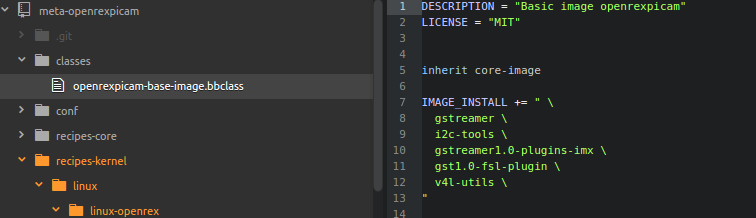
\includegraphics[width=1\linewidth]{packageclasse.png}
    \decoRule
    \caption{Emplacement et contenu de la recette de l'openrexpicam-base-image}
    \label{fig:arbor}
\end{figure}
